\documentclass{beamer}

\usepackage{fontspec}
\usepackage{xeCJK}
\setCJKmainfont[BoldFont=Noto Serif CJK TC Bold]{Noto Serif CJK TC}
\XeTeXlinebreaklocale "zh"
\XeTeXlinebreakskip = 0pt plus 1pt
\linespread{1.3}
\allowdisplaybreaks

%\newcommand{\weib}{\CJKfamily{weib}}
%\newcommand{\hkss}{\CJKfamily{hkss}}
%\newcommand{\hksy}{\CJKfamily{hksy}}
%\newcommand{\lth}{\CJKfamily{lth}}
\usepackage{color}
\usepackage{booktabs}
\usepackage{tabularx}
\usepackage{caption}
\usepackage{tikz}
\usepackage{verbatim}
\usepackage{pgfplotstable}
\pgfplotsset{width=12cm}
\pgfplotsset{height=7cm}
\pgfplotsset{compat=1.13}

\usetheme{EastLansing}
\usetikzlibrary{positioning}
\useinnertheme{rectangles}
\usefonttheme{professionalfonts}

\newcommand{\lw}{0.8mm}
\setbeamercovered{transparent}


%\AtBeginSection[]
%{
  %\begin{frame}<beamer>
	%\frametitle{報告大綱}
	%%\frametitle{RoadMap}
    %\tableofcontents[currentsection]
  %\end{frame}
%}

\title{Paper Report}
\subtitle{\textcolor[rgb]{0.00,0.50,1.00}{{Speech Processing \& Machine Learning Laboratory}}}
\author{徐瑞陽}
\date{2019/09/12}
\begin{document}

\begin{frame}
\maketitle
\end{frame}


\begin{frame}
  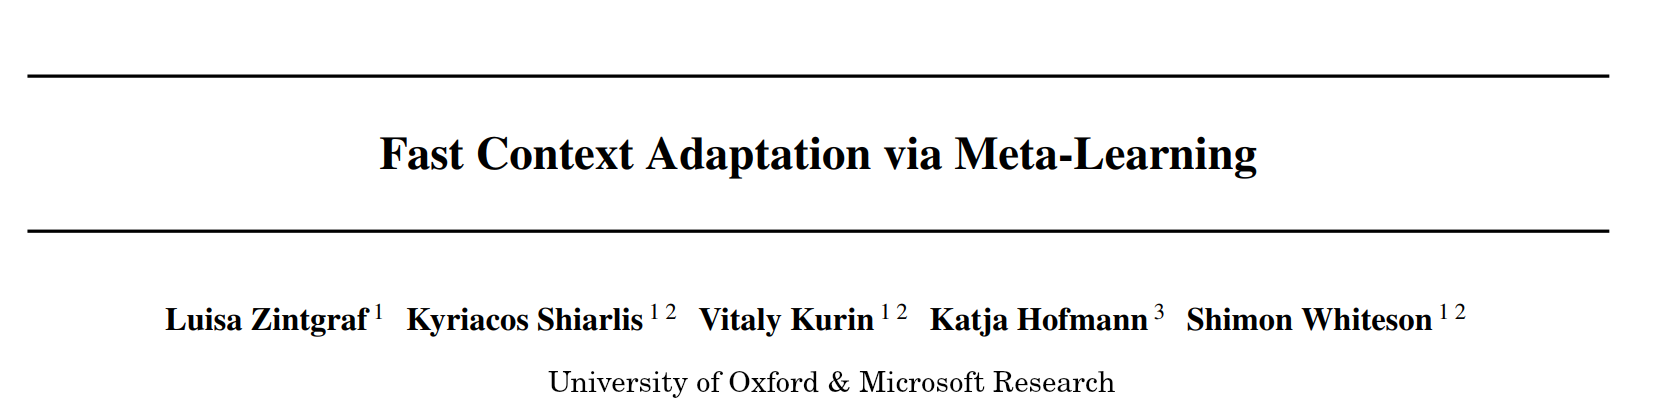
\includegraphics[width=\textwidth]{fig/CAVIA.png}
  \center ICML 2019
\end{frame}

\begin{frame}
  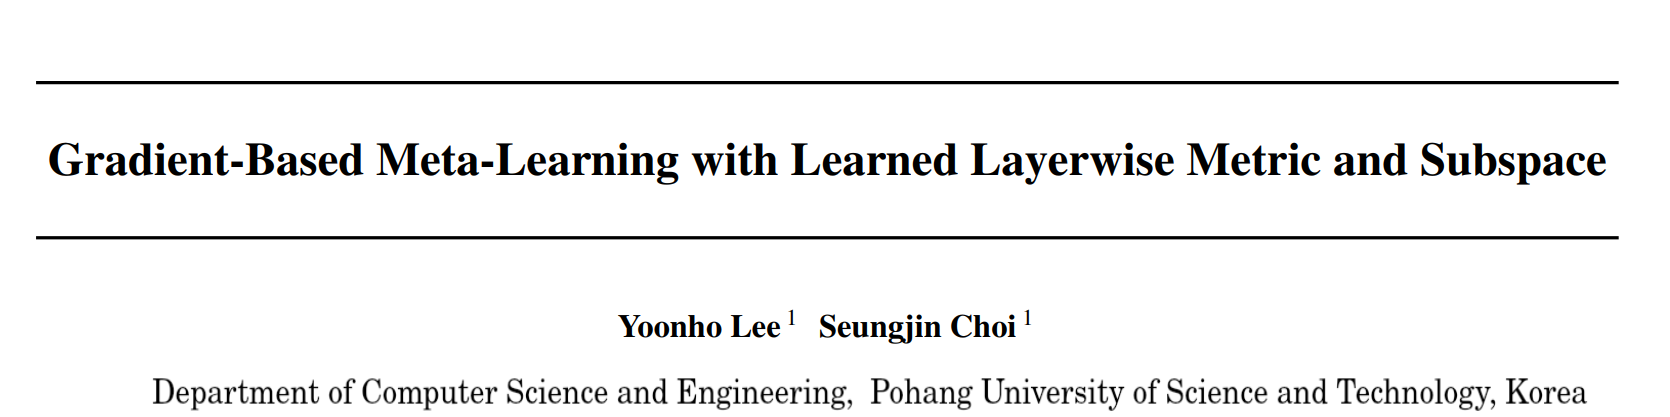
\includegraphics[width=\textwidth]{fig/title.png}
  \center ICML 2018
\end{frame}

\begin{frame}{Trends in Meta Learning}
  \begin{itemize}
    \item Task conditioning
    \item Parameter space warping
  \end{itemize}
\end{frame}

\begin{frame}
\frametitle{Outline}
\tableofcontents
\end{frame}

\section{Quick recap of meta learning}

\begin{frame}{Objective}
\[ \theta^\star = \arg \max_\theta \mathbb{E}_{\mathcal{D} \sim p(\mathcal{D}) }[\mathcal{A}_\theta(\mathcal{D})]\]

$\mathcal{A}$ depends on which application we want to learn \\ 
(e.g classification, regression... and MORE!!)
  
\end{frame}

\begin{frame}{Common Approaches\footnote{source: \href{http://metalearning-symposium.ml/files/vinyals.pdf}{Vinyals' talk at NIPS 2017}}}
  \begin{itemize}
    \item \textbf{Metric-based}
    \item Model-based: won't talk today
    \item Optimization-based
      \begin{itemize}
        \item Update rule: e.g optimizer
      \item \textbf{Initial weight} $\theta_0$
      \end{itemize}
  \end{itemize}
\end{frame}

\section{Task Conditioning}
\begin{frame}
  \begin{center}
    \LARGE{Task Conditioning}
  \end{center}
\end{frame}

\begin{frame}{Motivation}
  For different tasks, we still use
  \begin{itemize}
    \item Same structure: e.g feature encoder in metric-based approach
    \item Same parameter: e.g same $\theta_0$ in optimization-based approach
  \end{itemize}
  to adapt

  \begin{center}
    Can we exploit prior knowledge about tasks,\\ and adapt current task more effectively ?
  \end{center}
\end{frame}

\begin{frame}{Consider 2 extremes}
  Every task
  \begin{itemize}
    \item share same parameter $\theta$ to start
    \item have individual parameter (training from scratch)
  \end{itemize}
\end{frame}



\begin{frame}{Implementations of Task Conditioning}
  \begin{itemize}
    \item Learn \textbf{another} feature encoder as \textbf{condition of tasks} to get more useful representation before meta learning
      \begin{itemize}[<+->]
        \item TADAM: Use $\mu$ of class prototypes as task representation (NIPS 2018)
        \item CAML: Use ProtoNet offline learn an encoder to scale and shift $x_i$, then MAML (ICLR 2019)
        \item TAFE-Net: Use task embedding (sample image/ description) to generate weights of network used for prediction (CVPR 2019)
        \item Category Traversal
      \end{itemize}
  \end{itemize}
\end{frame}

\begin{frame}{Example: Overview of CAML}
  \center 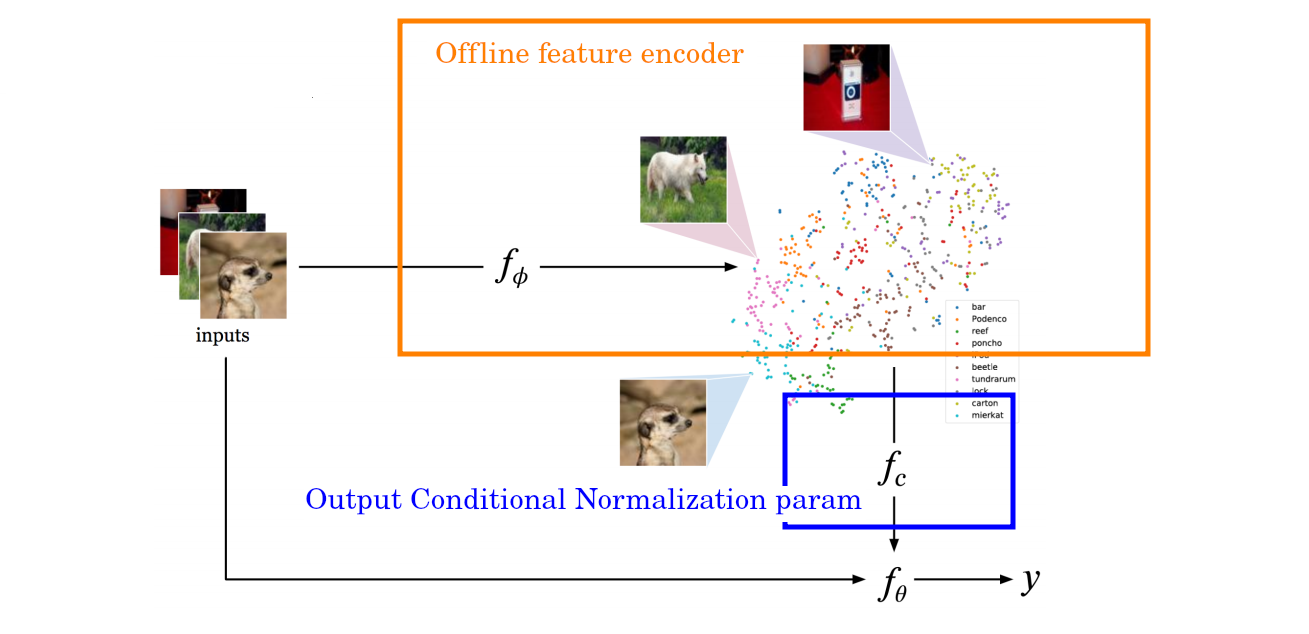
\includegraphics[width=1.0\textwidth]{fig/caml.png}
\end{frame}

\begin{frame}{Implementations of Task Conditioning}
  \begin{itemize}
    \item Cross-modality: \textbf{zero-shot concept} \\
      e.g use text embedding as additional input to learn prototype in ProtoNet (ICLR 2019)
  \end{itemize}
  \center 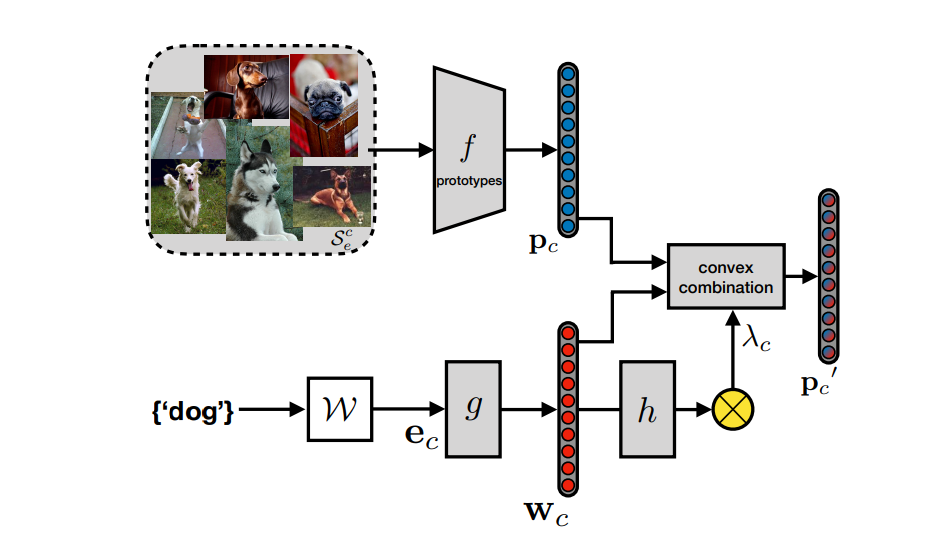
\includegraphics[width=0.7\textwidth]{fig/cross-modal.png}
\end{frame}

\begin{frame}{Implementations of Task Conditioning}
  \begin{itemize}
    \item Mask some parameter based on task representation
  \end{itemize}
  \center 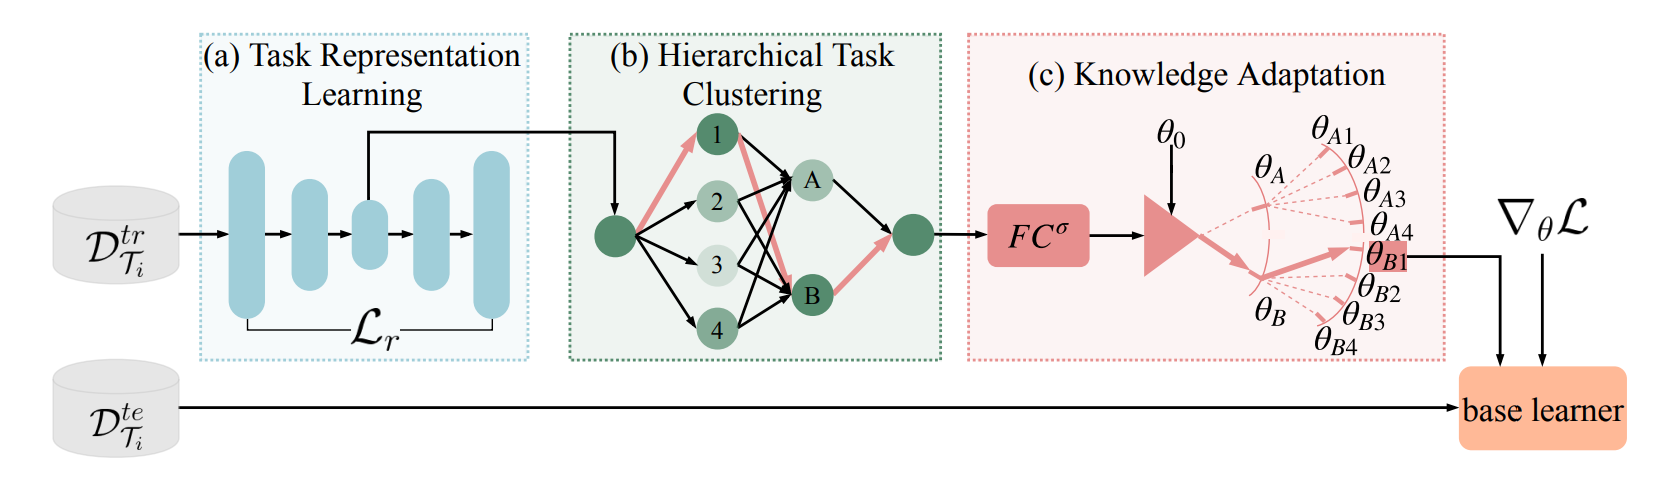
\includegraphics[width=\textwidth]{fig/hierarchical-meta.png}
\end{frame}

\begin{frame}{Results on 5-way 1-shot/5-shot on MiniImageNet}
  \center 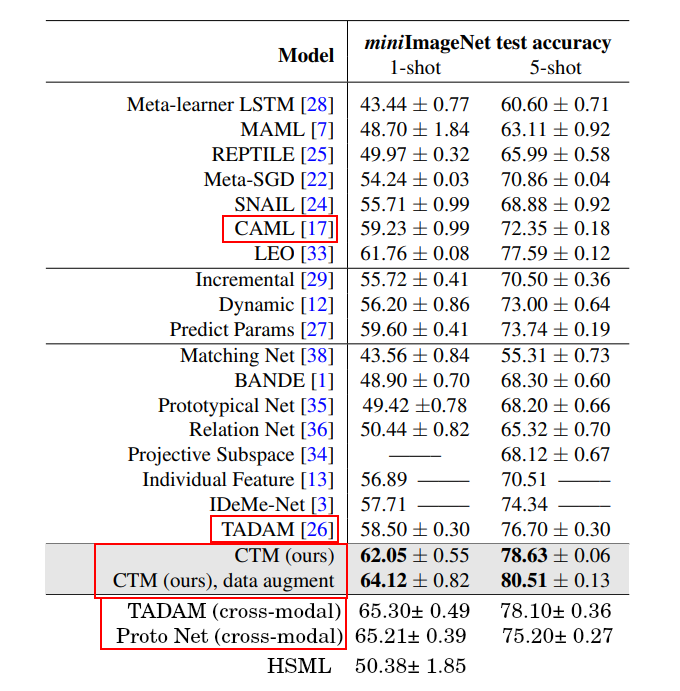
\includegraphics[width=0.6\textwidth]{fig/task-conditioning-result.png}
\end{frame}

\begin{frame}{Some Thoughts}
  \begin{itemize}
    \item Use \textbf{pre-trained} feature encoder as task representation extractor?
    \item Apply to Speech/NLP? depend on task definition!
  \end{itemize}
  %\begin{center}
  %\LARGE{What about applications in Speech/NLP} ?
  %\end{center}
\end{frame}

\section{Parameter Space Warping}
\begin{frame}
  \begin{center}
    \LARGE{Parameter Space Warping}
  \end{center}
\end{frame}

\begin{frame}{Motivation}
  Intuitively, meta learner model should have \textbf{more} capacity than learner model, but current optimization-based approach (e.g MAML) use same model/parameter for both of them\\
  \center operate in same parameter space is reasonable?
\end{frame}

\begin{frame}{Idea}
  Limit the freedom of task learner by fixing some param during adaptation
  \center 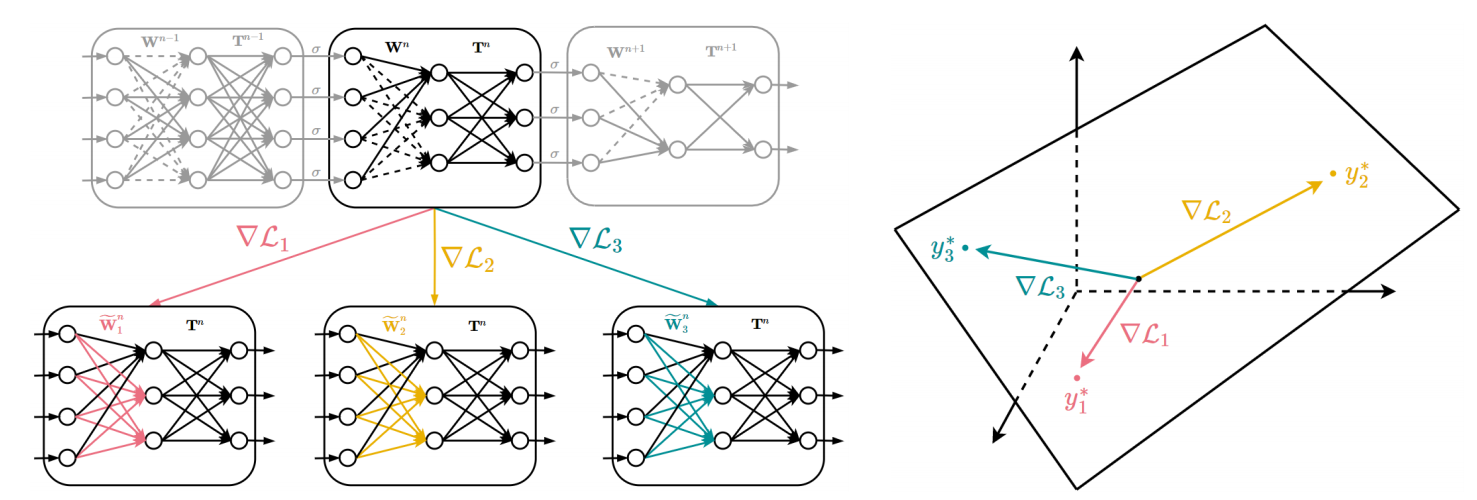
\includegraphics[width=1.0\textwidth]{fig/space-warp.png}
\end{frame}

\begin{frame}{Implementations of Parameter Space Warping}
  We have 2 sets of parameters
  \begin{itemize}
    \item $\phi$: param shared across and fixed during adaptation,\\ updated in outer loop (\textbf{meta})
    \item $\theta$: param for adaptation (but initial value shared across task), updated in inner loop
  \end{itemize}
\end{frame}

\begin{frame}{Key Questions for Implementations}
  \begin{itemize}
    \item How to determine param belong to which set?
      \begin{itemize}
        \item pre-defined
        \item learned
      \end{itemize}
    \item Which \textbf{warp} module should use?
      \begin{itemize}
        \item simple feed-forward
        \item complicated structure (like recurrent structure)
      \end{itemize}
  \end{itemize}
\end{frame}

\subsection{CAVIA}
\begin{frame}{CAVIA}
  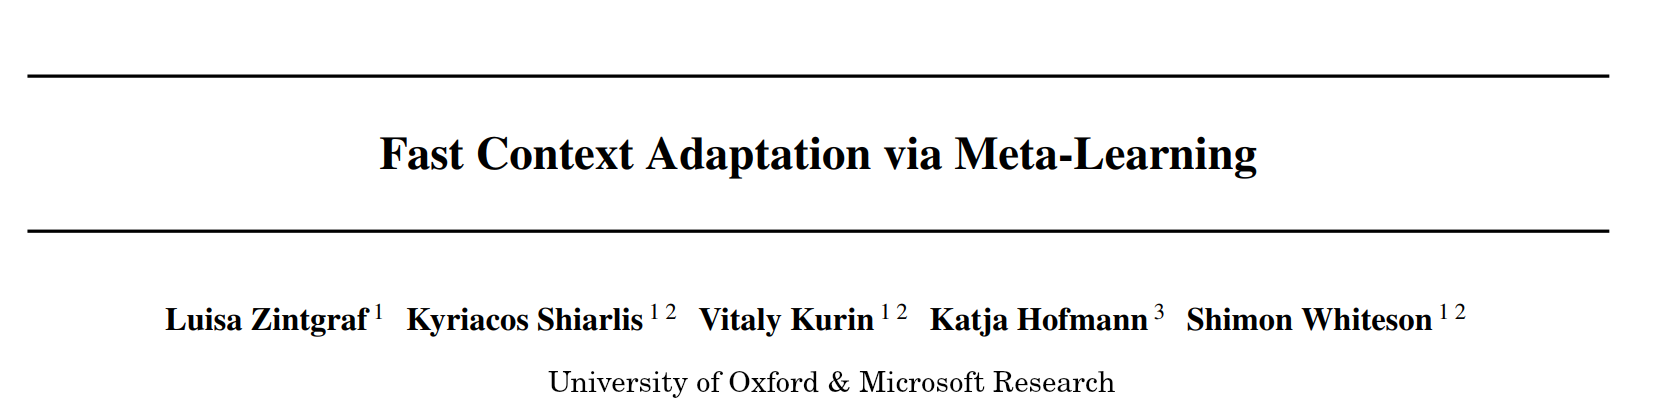
\includegraphics[width=\textwidth]{fig/CAVIA.png}
  \center ICML 2019
\end{frame}

\begin{frame}{Architecture of CAVIA}
  \begin{itemize}
    \item pre-defined meta param set
    \item feed-forward warp module
  \end{itemize}
  \center 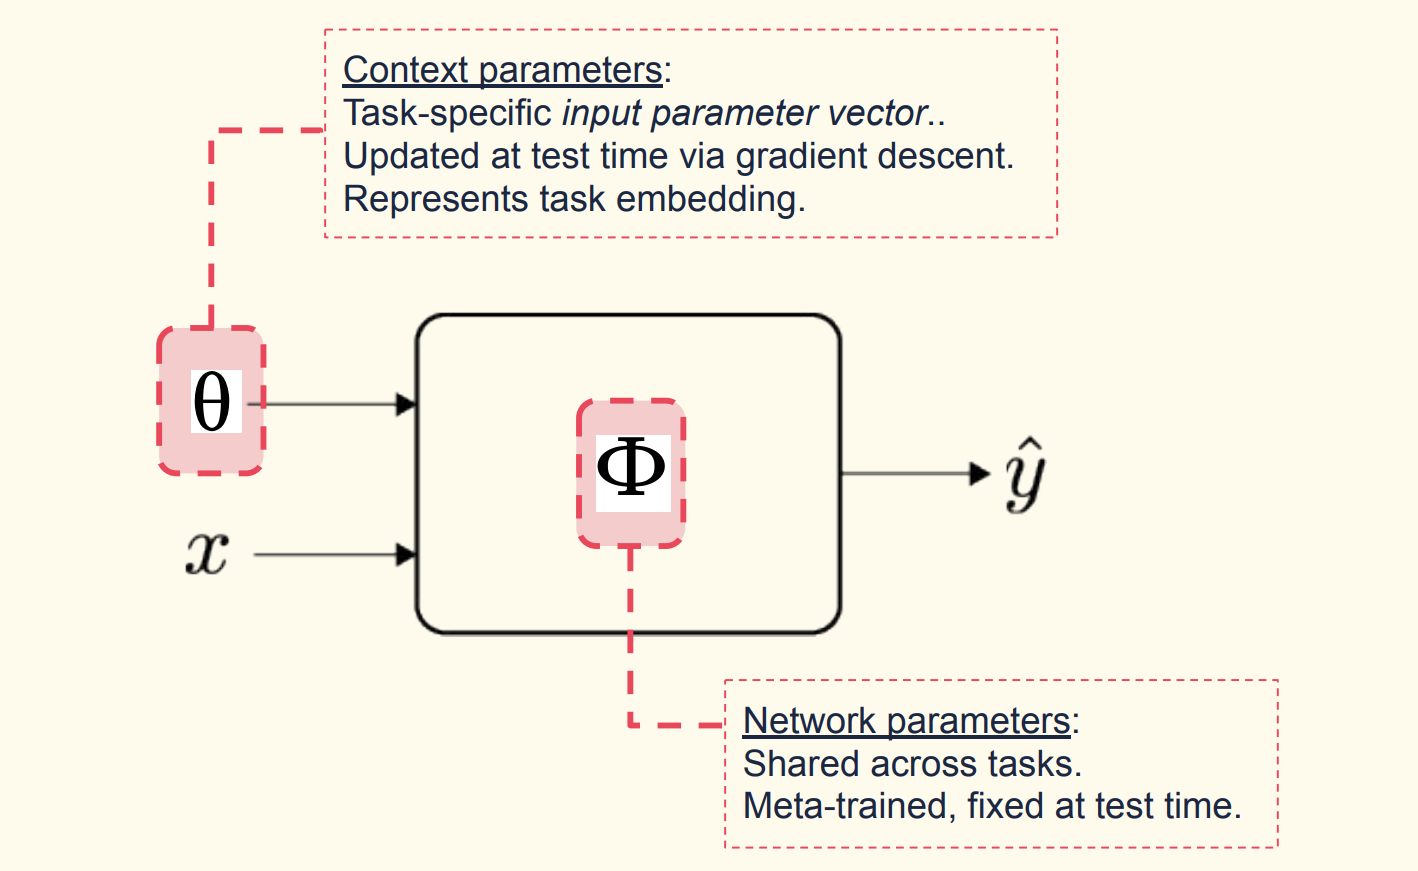
\includegraphics[width=0.7\textwidth]{fig/CAVIA-idea.png}
\end{frame}

\begin{frame}{Update Rule of CAVIA}
  \begin{itemize}
    \item prediction given network: $f_{\phi,\theta_0}(x)$
    \item loss of task $i$: $\mathcal{L}_{T_i}(f_{\phi,\theta_0}(x),y)$
    \item training set of task $i$: $\mathcal{D}_i^{train}$, testing set: $\mathcal{D}_i^{test}$
    \item $\theta_0 = \mathbf{0}$
  \end{itemize}
\end{frame}
\begin{frame}{Update Rule of CAVIA}
  \begin{block}{Inner loop udpate}
    \[\theta_i = \theta_0 - \alpha \nabla_{\theta} \frac{1}{|\mathcal{D}_i^{train}|}\sum_{(x,y) \in \mathcal{D}_i^{train}}\mathcal{L}_{T_i}(f_{\phi,\theta_0}(x),y)\]
  \end{block}

  \begin{block}{Outer loop update}
    \[ \phi \leftarrow \phi - \beta \nabla_{\phi}\frac{1}{N} \sum_{T_i \in \mathcal{T}} \frac{1}{|\mathcal{D}_i^{test}|} \sum_{(x,y) \in \mathcal{D}_i^{test}} \mathcal{L}_{T_i}(f_{\phi,\theta_i}(x),y)\]
  \end{block}
  $N$: meta batch size of tasks $\mathcal{T}$
\end{frame}

\begin{frame}{Experiment: Sine Curves Regression}
  A task 
  \begin{itemize}
    \item defined by amplitude ($\sim U(0.1,0.5)$) and phase ($\sim U(0, \pi)$)
    \item $10$ labeled data points given during adaptation
  \end{itemize}
  Model
  \begin{itemize}
    \item NN with 2 layers with 40 nodes
    \item Number of additional input params $\theta$: $2 \sim 50$
  \end{itemize}
\end{frame}

\begin{frame}{Experiment: Sine Curves Regression}
  \center 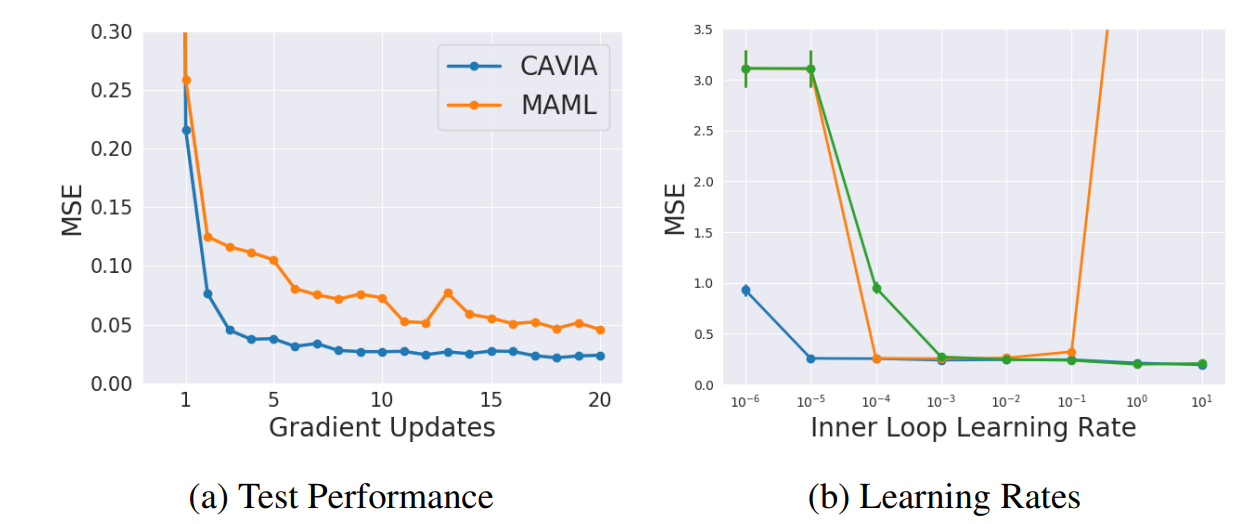
\includegraphics[width=1.0\textwidth]{fig/caml-sine-result.png}
  Green line: also meta-learn $\theta_0$ (rather than set to $\mathbf{0}$)  
\end{frame}

\subsection{MT-Net}
\begin{frame}{MT-Net}
  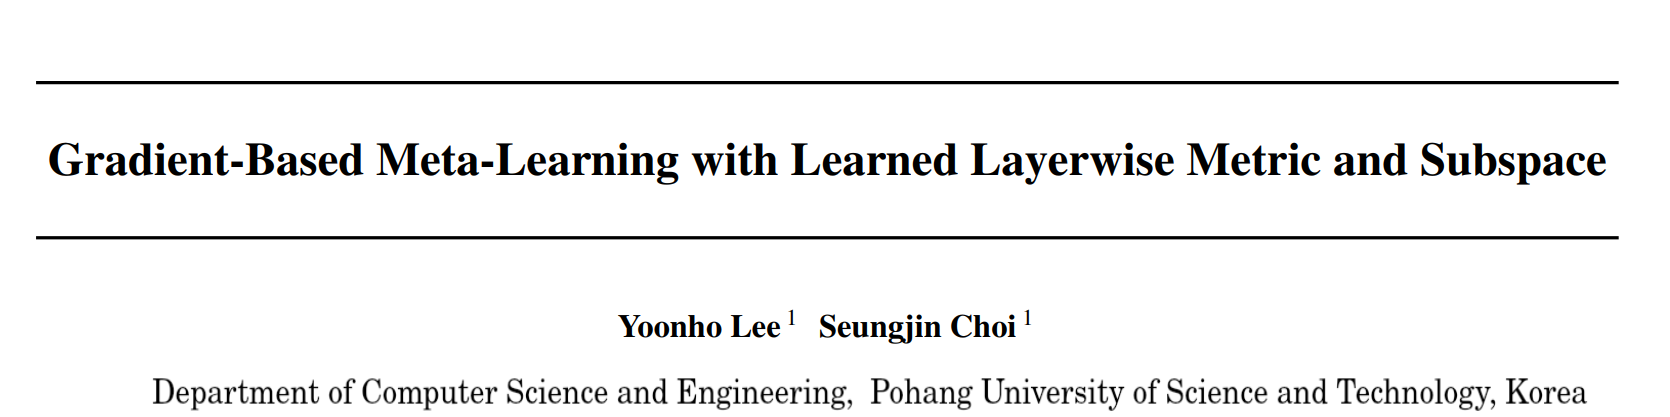
\includegraphics[width=\textwidth]{fig/title.png}
  \center ICML 2018
\end{frame}

\begin{frame}{Architecture of MT-Net}
  \begin{itemize}
    \item \textbf{learned meta param set}: see next slide
    \item feed-forward warp module
  \end{itemize}
  \center 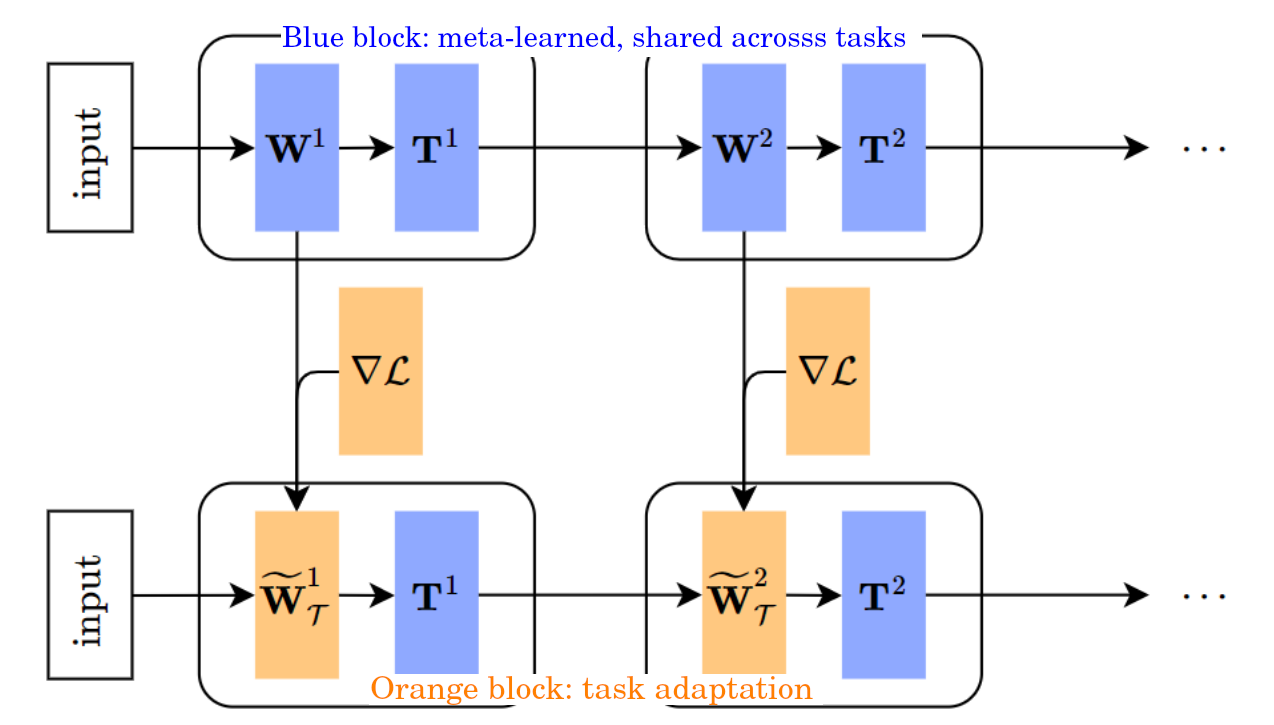
\includegraphics[width=0.8\textwidth]{fig/MT-idea.png}
\end{frame}

\begin{frame}{Architecture of MT-Net}
  \begin{itemize}
    \item T-net: last slide, learns a metric in activation space
    \item MT-net: additionally learned which subset of params should be adaptated
  \end{itemize}
  \center 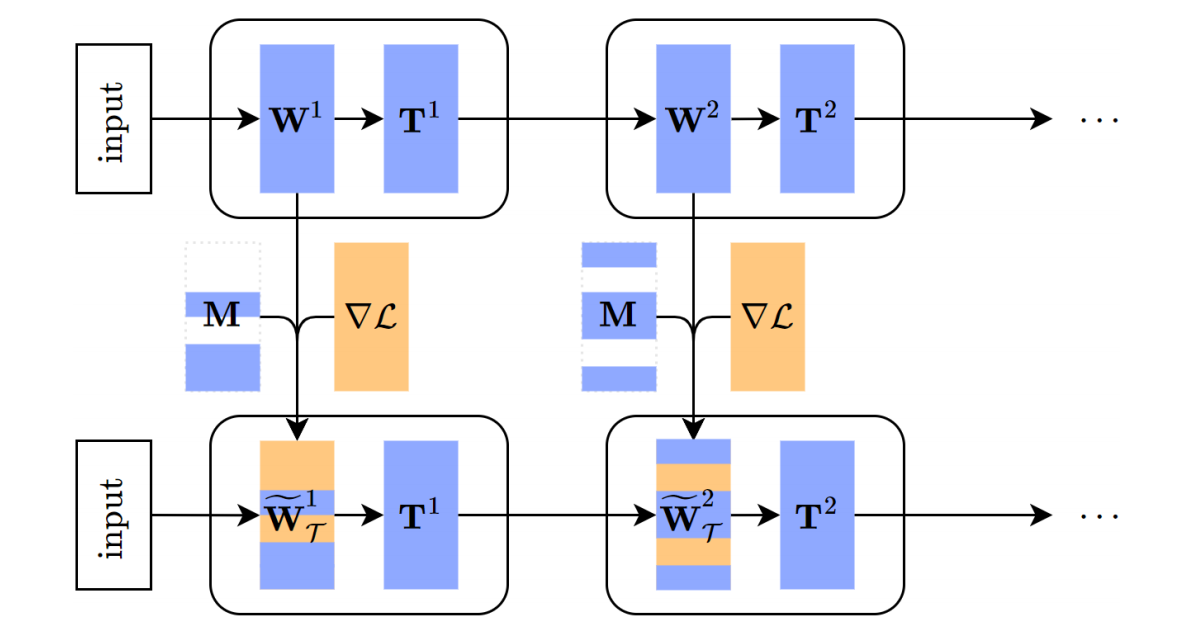
\includegraphics[width=0.8\textwidth]{fig/MT-idea2.png}
\end{frame}

\begin{frame}{More on mask $M$}
  \begin{itemize}
    \item $W$ is $m \times n$ matrix, T is $n \times n$ matrix
    \item $M = [\mathbf{m_1},\cdots,\mathbf{m_n}]^\top$
    \item $\mathbf{m_j}^\top \sim Bern\Big( \frac{\exp(\zeta_j)}{\exp(\zeta_j) + 1} \Big) \mathbf{1}^\top$
  \end{itemize}
\end{frame}

\begin{frame}{Update Rule of MT-Net}
  \begin{itemize}
    \item meta param $\phi = \lbrace \underbrace{W^1,\cdots,W^L}_{\theta_W},\underbrace{T^1,\cdots,T^L}_{\theta_T},\underbrace{\mathbf{\zeta^1},\cdots,\mathbf{\zeta^L}}_{\theta_\zeta} \rbrace$
    \item param for adaptation $\theta = \lbrace \underbrace{W^1,\cdots,W^L}_{\theta_W} \rbrace$
  \end{itemize}

  Note
  \begin{itemize}
    \item same rule as CAVIA
    \item use \texttt{Gumbel-Softmax} estimator to differentiate through sampling of masks
  \end{itemize}
  %\begin{block}{Outer loop update}
    %\[ \phi \leftarrow \phi - \beta \nabla_{\phi}\frac{1}{N} \sum_{T_i \in \mathcal{T}} \frac{1}{|\mathcal{D}_i^{test}|} \sum_{(x,y) \in \mathcal{D}_i^{test}} \mathcal{L}_{T_i}(f_{\phi,\theta_i}(x),y)\]
  %\end{block}
\end{frame}

\begin{frame}{More on MT-Net}
  Consider the output changes as follows, denote $A=TW$

  \begin{block}{Output change}
    \[ \mathbf{y}^{\text{new}} = \mathbf{y} - \alpha (T \odot M_T^{\top}) (M_T \odot T^{\top}) \nabla_A \mathcal{L}_{\mathcal{T}}\mathbf{x} \]
  \end{block}

  \begin{itemize}
    \item $T$ controls the step size (make model more lr-agnostic)
    \item $M$ defines the task-specific \& task-mutual neurons
  \end{itemize}
\end{frame}

\begin{frame}{Experiment: Sine Curves Regression}
  Same setting as CAVIA
  \center 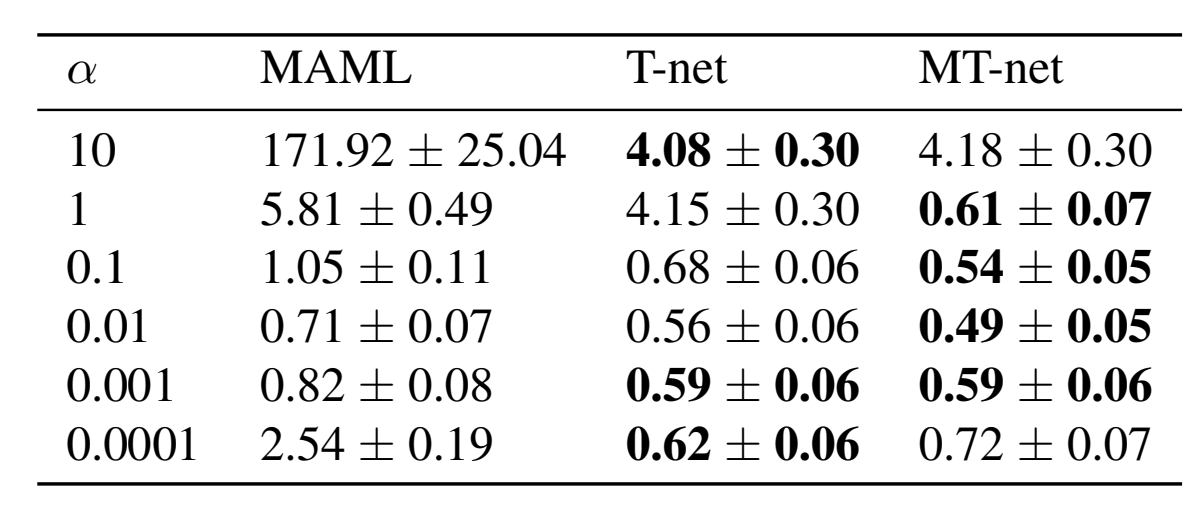
\includegraphics[width=0.8\textwidth]{fig/MT-sine.png}
\end{frame}

\begin{frame}{Experiment: Polynomial Regression}
  A task
  \begin{itemize}
    \item defined by $\sum_{i=0}^n c_i x^i$
    \item $n \in \lbrace 0, 1, 2 \rbrace$
    \item $c_0, c_1, c_2 \sim U(-1,1)$
    \item $10$ labeled data points given during adaptation
  \end{itemize}

\end{frame}

\begin{frame}{Experiment: Polynomial Regression}
  \center 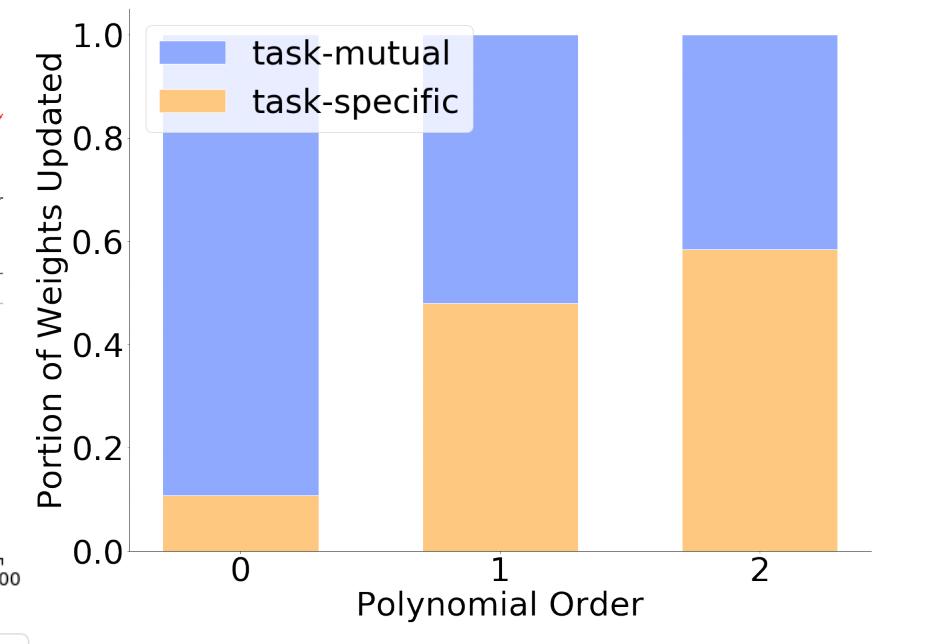
\includegraphics[width=0.7\textwidth]{fig/MT-poly.png}
  \center Observation: dimension of the learned subspace reflect the underlying complexity of tasks
\end{frame}

\subsection{Warped Gradient Descent}
\begin{frame}{Warped Gradient Descent}
  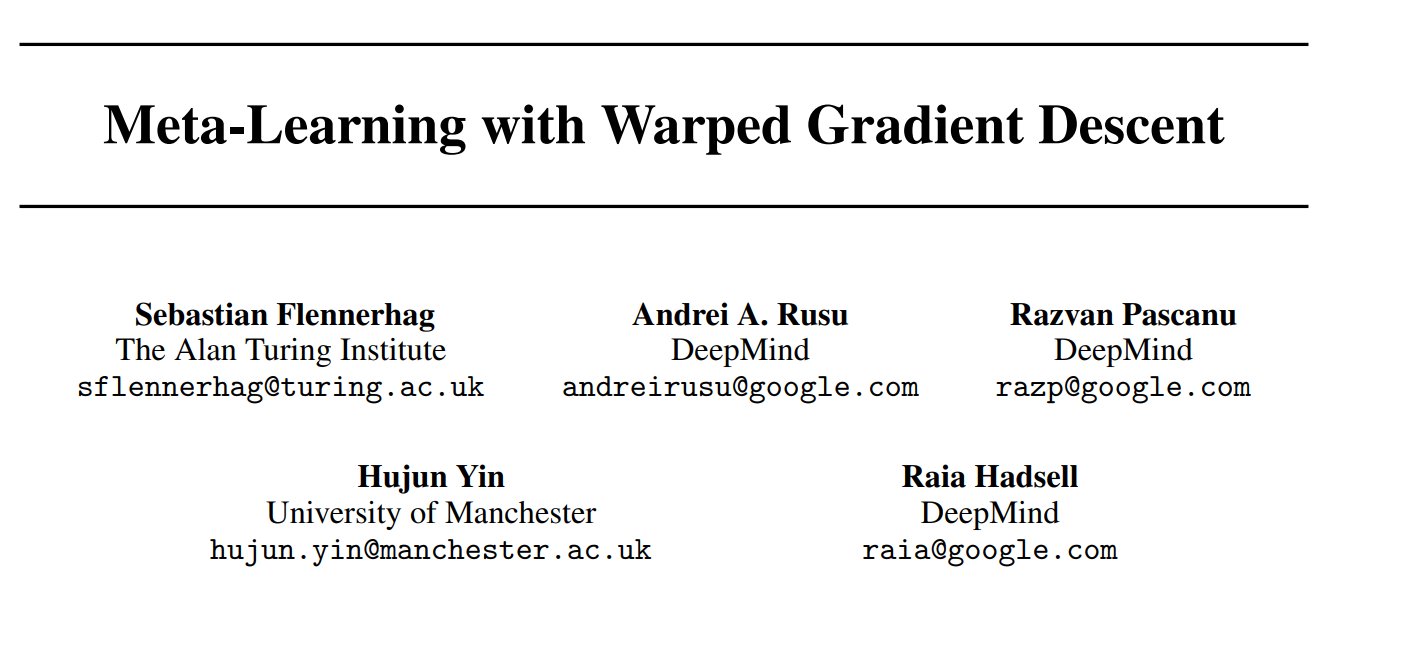
\includegraphics[width=\textwidth]{fig/Warp-meta.png}
  \center 8/30 on Arxiv
\end{frame}

\begin{frame}{Architecture of Warped-GD}
  \begin{itemize}
    \item predifined/learned meta param set
    \item complicated warp module
    \item define $\mathcal{L}_{meta}, \mathcal{L}_{task}$ individually
  \end{itemize}
  %\center 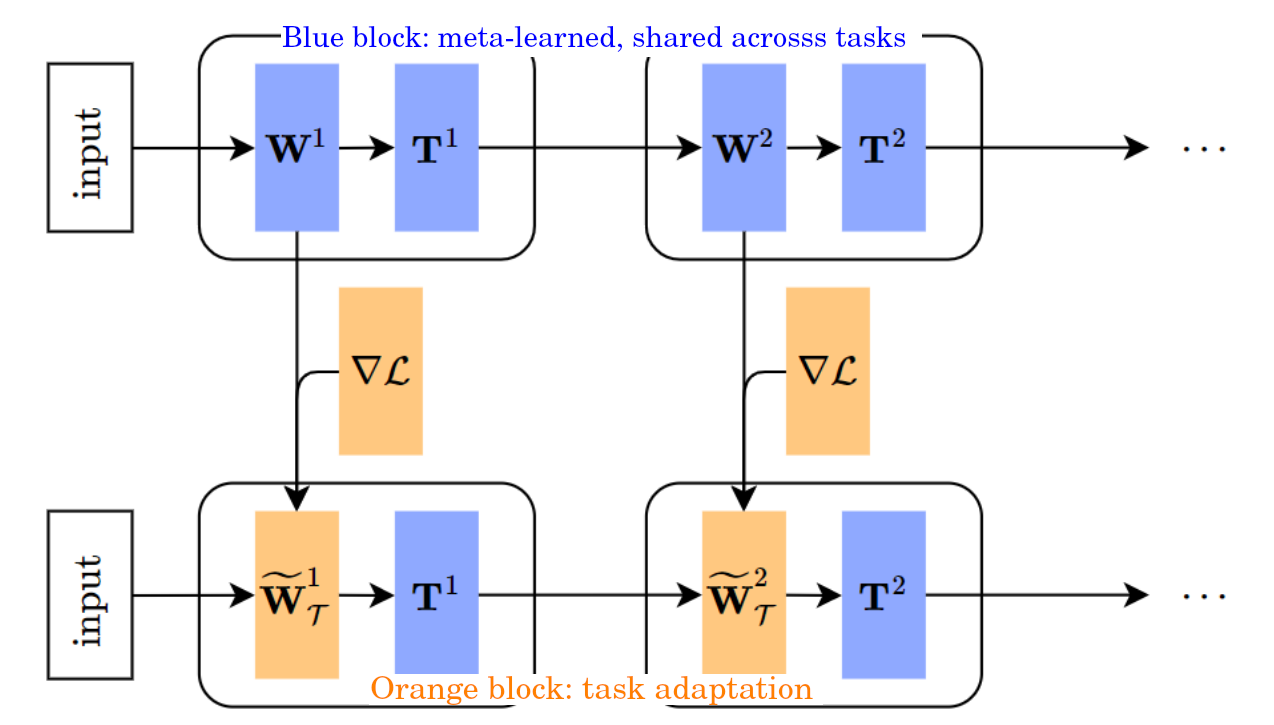
\includegraphics[width=0.8\textwidth]{fig/MT-idea.png}
\end{frame}

%\section{MISC}
\begin{frame}
	\begin{center}
    %\weib{\LARGE{謝謝聆聽!}}
    \LARGE{Questions?}
	\end{center}
\end{frame}


\subsection{Appendix}
\end{document} 
